\label{ch:results}
This chapter deepens and extends some of the terms given in chapter \ref{ch:methods} and investigates them with respect to automotive. The chapter is structured into five main section, entitled \emph{SoA in embedded systems (Embedded SoA)}, \emph{SoA in automotive}, \emph{safety services}, \emph{service development process} and \emph{use case scenario}. 

The first section deals extensively with the application of the service oriented design paradigm in embedded system and highlights the challenges this approach has to face when it has to face certain safety requirements. Moreover, the differences to ``conventional SoAs'' as web application is investigated in detail. In the second section various examples of services, relevant for functional safety are described in detail, and their intended functionality, as well as possible implementations in terms of architecture is presented. The final part consists of a simplified use case, dealing with the design of an \emph{error detection service} with respect to the design phases \emph{service investigation/ planning}, \emph{service inventory analysis}, \emph{service oriented analysis} and \emph{service oriented design}.

Most of the findings and concepts in this chapter are (not yet) covered in literature, but are the result of numerous meetings and discussions at \textbf{VIRTUAL VEHICLE Research Center} during April to July 2015.







\section{SoA in Embedded Systems (Embedded SoA)}
\label{sec:soa-in-embedded-systems}

The service oriented design paradigm was originally designed for the application on the Internet, which offered ideal prerequisites for this kind of architectural style. An underlying network for interconnection was already present and time constraints are no concern, for delays are unlikely to cause a disaster. Thus, it is no surprise that web services are the application area, where SoA has scored the highest market penetration \cite{rodrigues2011} \cite{buckl}.


\subsection{Drawbacks in Embedded Systems}
In contrast to web services, ESs consist of numerous interconnected nodes, with diverse measurement-, steering-, or computation capabilities. Accordingly, they have to face additional challenges like \emph{limited resources}, \emph{different complexity of hardware}, \emph{time constraints} and others \cite{scholz} \cite{sommer}: 

\begin{description}
\item [Limited resources.]
One obvious major drawback of ESs are the quite limited resources, which are designed for highly specialized purposes and lack computation power as well as storage capacities \cite{rodrigues2011} \cite{scholz} \cite{sommer}.

\item [Different levels of complexity.]
The complexity of hardware in ESs varies greatly. The implemented components may include very primitive sensors with few capabilities, but also very advanced nodes like MPSoCs \cite{scholz} \cite{sommer}. In other words, there are high level \emph{information systems services}, as well as low level generic \emph{embedded system services}. A SoA has to deal with the connection and integration of them \cite{rodrigues2011}. This task gets aggravated if SoAs in ESs become interconnected with high level SoAs like web applications.

\item [Event- and data-driven.]
In contrast to web services, an ES disposes of a network with (many) sensors. Thus, the ad-hoc \emph{request-response} message pattern, which is common for web services, cannot be simple adopted for the \emph{event- and data driven} ES \cite{sommer}.

Instead, the communication in those is conducted mainly by a \emph{fire and forget} scheme: A sensor measures some data and publishes it to all connected services, which have to decide on themselves, whether the received data is relevant and how to process the received information \cite{sommer}.

\item [Lifespan of services.]
Another difference to web services is the lifespan of services. While web services are used to work only a limited number of hours (or even just minutes), the services in ESs could have application times of multiple years, or may even last for the lifespan of the system \cite{buckl}.

\item [Dynamic character.] 
The components of a SoA show dynamic characteristics: ``new nodes may enter the network, existing nodes may fail and network characteristics can change over time, especially if wireless communication media are used'' \cite{sommer}. This could become an issue, for ESs where the set of implemented components is usually determined at assembly time.

\item [Time constraints.]
ESs are \emph{time-critical}, meaning that computation must be conducted within a given time window in order to allow the correct operation of the system. Especially in a safety-critical system like a vehicle, which is used to operate at high velocities, a violation of those time constraints could cause serious incidents.
\end{description}

These obstacles are the reason why web services and safety-critical embedded systems are often considered as non-related areas \cite{rodrigues2011}. Nevertheless, Sommer et al. mention various benefits which come with the application of the SoA design philosophy in ESs: 
\begin{itemize}
\item Decoupling configuration from environment, 
\item Improvement of reusability,
\item Improvement of maintainability,
\item Higher level of abstraction,
\item Enhanced interoperability and
\item More interactive interfaces between devices and information system \cite{buckl}.
\end{itemize}

To sum up, the SoA paradigm has to overcome many serious drawbacks if applied in ESs, but at the same time it offers numerous advantages and possibilities, which are just not possible with current systems. 



\subsection{Embedded SoA}
There is no uniform denomination for SoAs in ESs throughout literature. Thus, it is referred to by the term \emph{Embedded SoA} (abbreviated as ESoA) for the scope of this thesis.

The following definition is the result of intense investigation in this area and extends the definition from section \ref{ch:soa}:

\begin{myquote}
The Embedded SoA works at a lower, very hardware oriented level, with a predefined and unchanging set of component.

The conventional SoA is located above the embedded SoA and connected through various interfaces.
\end{myquote}

With respect to the example of a vehicle, the ESoA operates on elements like the power train, various devices (sensors, actuators, controllers, etc.), while the SoA level contains the vehicle as overall system. With other vehicles and environmental components it may form a SoS.

Regarding the \mbox{ISO 26262 standard}, the requirements for ESoA can be related to \textbf{Part 3: Concept phase}, and the SoA to \textbf{Part 4: Product development at the system level} as depicted in figure \ref{fig:soa-and-esoa}.


\begin{figure}[!htbp]
\centering
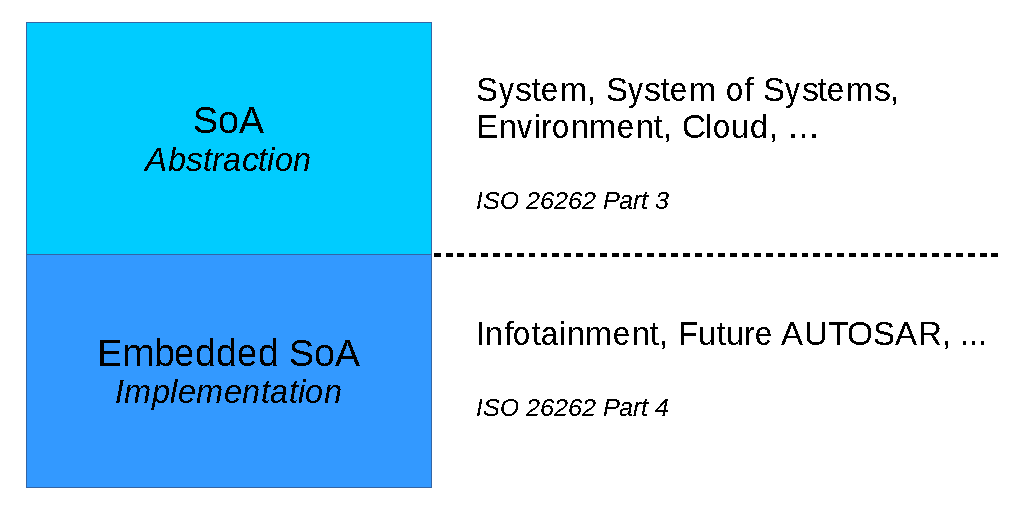
\includegraphics[scale=0.8]{soa-and-esoa.pdf}
\caption{Relation of conventional SoA to Embedded SoA.}
\label{fig:soa-and-esoa}
\end{figure}







\section{SoA in Automotive}
\label{sec:soa-in-automotive}

In the future of automotive all vehicles will, most likely, be interconnected with each other and also with the environment. This is a necessary prerequisite for acting autonomously, e.g. detecting whether the traffic lights at a crossing are green. Within this document those futuristic vehicles are referred to as \emph{connected cars}.

The opportunities and advantages of the SoA approach are described extensively in \ref{sec:soa-in-embedded-systems} and \ref{ch:soa}. In terms of vehicles, the major advantage would be the possibility to reduce the quantity of computation hardware. At present time, each component disposes of his own dedicated hardware for conducting computations. Although it is unused for the majority of time, it comes with a lot of extra weight, what is a major violation of the guideline stated in \cite[p.7]{marwedel}, ``Embedded systems should exploit the available hardware architecture as much as possible.'' The SoA approach might not only reduce the weight, but thereby also the complexity and costs of the overall vehicle. In today's automotive systems it is common practice that each vendor uses his own proprietary network and additional hardware, prohibiting the application of hardware components from another vendors \cite{sommer}.

However, there are some obstacles which prevent the application of the SoA paradigm in vehicles right now. On the one hand, those are the strict regulations in connection with safety critical real-time systems like vehicles \cite{kum}. With respect to automotive there are not even regulations, addressing SoA, yet. On the other hand, there are pure technical constraints. The \mbox{AUTOSAR} architecture, which is widely applied today, is not constructed for dynamic reconfiguration or binding of services at runtime, but everything has to be specified at building time. Nevertheless, there is already an approach by \mbox{AUTOSAR}, denoted \emph{Future \mbox{AUTOSAR}}, dealing with this very issue. Unfortunately, the actual implementation in mass produced vehicles is quite some time ahead.

To sum up, it might take some time before the design paradigm will be used for the lower, hardware-oriented layers of the ESoA. Instead, it would be a promising approach for higher layers like the SoS. The vehicle as system could offer certain services to its environment and the other way round. A good example, which has been mentioned before, are traffic lights. If the the traffic lights in Germany use another service as the ones in Austria, a SoA could enable the dynamical binding of the new service, when a vehicle approaches the border.


\subsection{Location of the service repository}
The description of the term service repository is covered in \ref{sec:structure_of_soa}. Nevertheless, questions arose concerning its location and actual implementation with respect to automotive. This section covers the findings concerning this matter.

For SoAs in automotive it is very likely that there will emerge various, physically and logically, distributed repositories. One repository inside of every vehicle, containing all the services provided by the vehicle itself and used by the vehicle itself. This repository obviously has to be located inside the vehicle, for it has to be also available when the vehicle is operating in urban regions or when it is just not able to connect to its environment. These repositories may be referred to as \emph{local service repositories}. Examples for services in this repository are services which are closely connected to hardware components like sensor measurements or communication services, but also safety services for fault- and error detection, which need to be available whenever the vehicle is operated.

The counterpart to the local service repository is denoted \emph{external service repository}. This could also be physically distributed on various server clusters and should hold mostly services which are needed for interacting with the environment. To connected cars, it could provide all the services needed for managing the traffic. In order to stick to the previous example, a service at this repository could be dedicated to managing the traffic lights of a particular city or zone. If it is bound by a vehicle operating in this zone, it should then be able to decide automatically, whether it has to stop at an intersection.

Other services which could be located in this repository are \emph{update services}. If an update for an existing service in the local repository is available, the vehicle could detect this automatically and subsequently load and install the service in question.


\subsection{Service Contract}

The service contract (cf. section \ref{sec:service_structure}) is the complete and extensive description of the service and with respect to automotive it should also contain documentation from AUTOSAR, the \mbox{ISO 26262} standard and documentation regarding functional safety. One of the goals of \textbf{Work Package 1} of the EMC2 project to extend the service contract by a functional safety part.

At the beginning of a service development process, the contract exists just as an empty template, which gets filled more and more as the development advances. A template, which should be used for the development of services in the automotive industry is provided by the Arrowhead project.













\section{Safety services}

For most safety-critical ESs security is also an important issue. Accordingly, most of the provided services must be fault tolerant and secure at the same time.

Functional safety is directly related to availability (cf. section \ref{sec:availability}) and thus the overall safety can be increased by increasing the availability \cite{turek2011}. The availability, in turn, can be increased by services for failure detection, error detection and error masking, which also enable recovery from errors.

In the following sections, the interference and connection of safety and security services is analysed, before the functional principles of a few selected safety services is presented in detail.

\subsection{Relation of Safety and security services}

In vehicles it is not really possible to distinguish safety functions from ``normal'' functions, because a malfunction in any functionality could lead to a disaster \cite{iso26262:course2}. Accordingly, all services are also considered to be safety-critical.

Since future vehicles are planed to be always connected to the outside world, security must also be taken into account, because a malicious attack on the system could be equally disastrous. In terms of security, there will be dedicated services which take are of authentication, permission management and comparable functionalities.

Most of those safety- and security services cannot be assigned entirely to one discipline, but have overlapping responsibilities, as depicted in figure \ref{fig:safety-and-security-services}. According to various findings, this effects especially the services for \emph{authentication}, \emph{memory protection} and \emph{failure detection}.

\begin{figure}[!htbp]
\centering
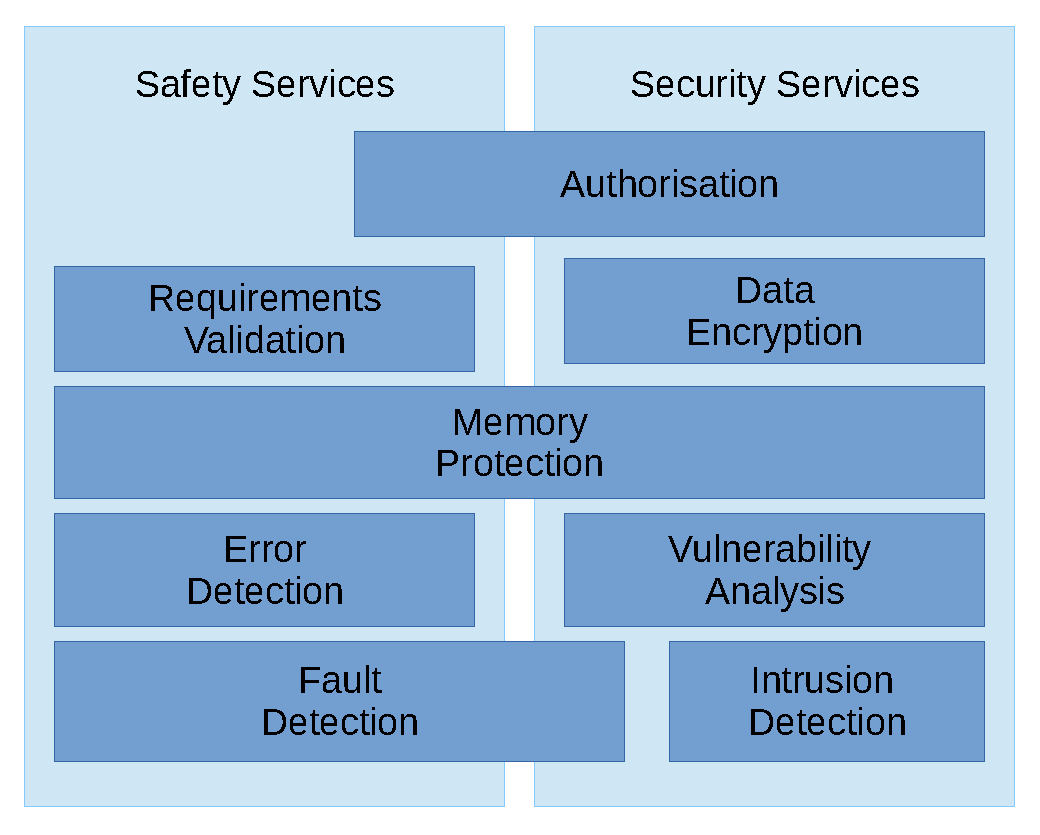
\includegraphics[scale=0.6]{safety-and-security-services.pdf}
\caption{Classification of various services into safety and security services.}
\label{fig:safety-and-security-services}
\end{figure}




\subsection{Failure Detection Service}

A Fault Detection Service (FDS) is a service which is capable of detecting faults, and eventually, depending on its implementation, also \emph{control flow errors}. Control flow errors are errors, which lead to a wrong execution sequence of the instructions of a service. Technically, the FDS can be implemented as simple timer circuit with a specified threshold time. If this limit is reached, it changes its state in order to trigger further actions, like restarting a component or activating another safety service [7]. The advantage of the FDS is the simple design, which reduces the additional complexity of the overall system, as well as the costs. Concerning the functional principle, there exist different designs with increasing complexity, which can provide, for example, a certain time window for the response [7].


\begin{figure}[!htbp]
\centering
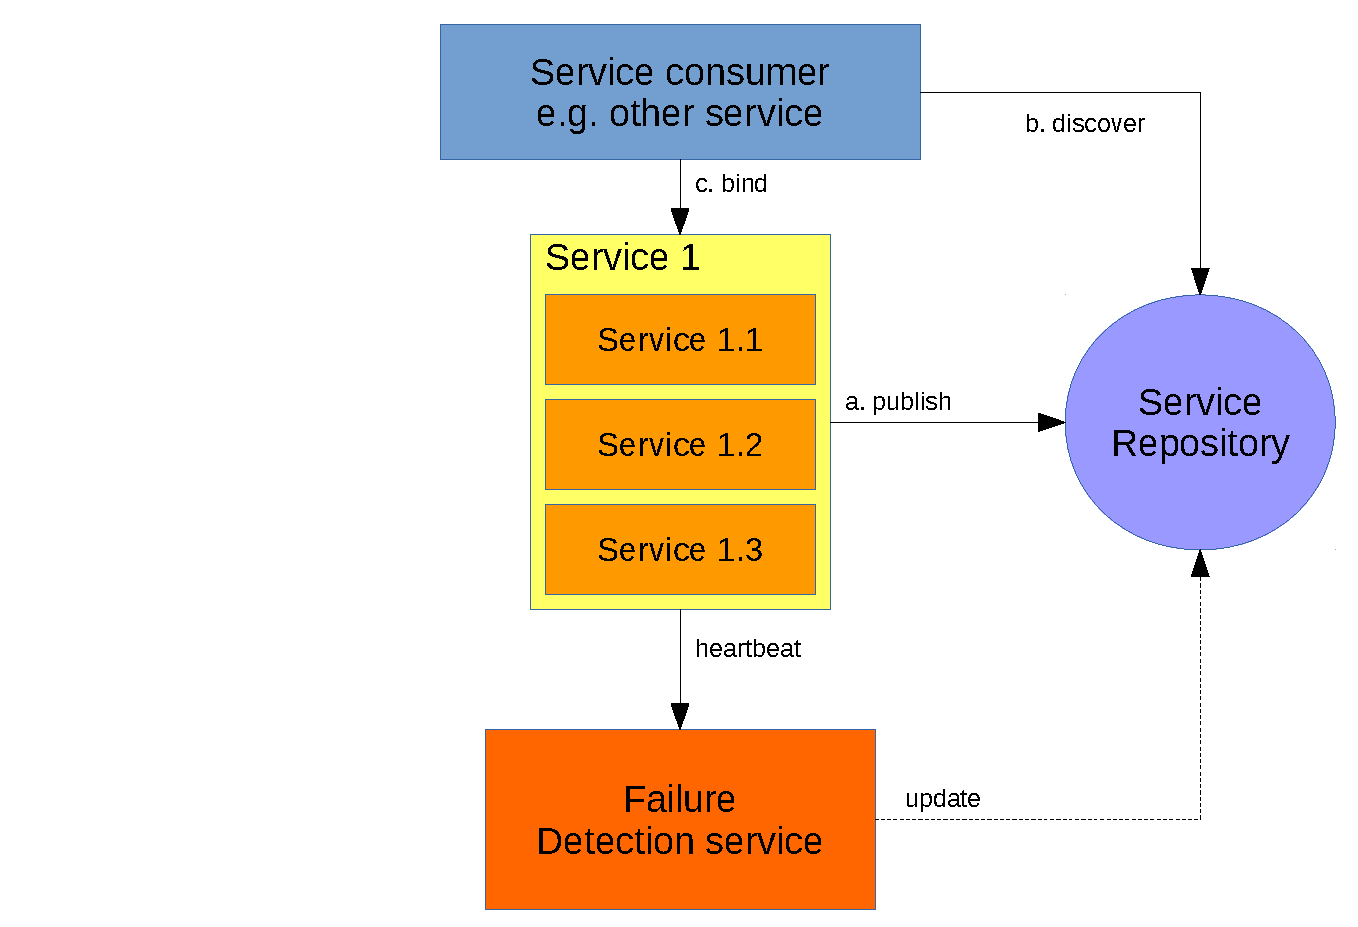
\includegraphics[width=\textwidth]{fault-detection-service.pdf}
\caption{Example architecture for an \emph{fault detection service}, like a WDT.}
\label{fig:fault-detection-service}
\end{figure}

In the following, a fault detection service is described by means of its most prominent representative, the so called \emph{Watchdog Timer (WDT)}.

As suggested by the name, the WDT is based on a timer, which gets reset every time, a heartbeat signal from the observed service is received. There three different basic designs: the \emph{Standard Watchdog Timer}, the \emph{Windowed Watchdog Timer} and the \emph{Sequenced Watchdog Timer} \cite{elattar2007}.


\begin{description}
\item [Standard Watchdog Timer.]
With this basic setup, the service mirrored by the WDT periodically sends a simple heartbeat signal, which resets the timer and indicates that the service is alive and active. If a predefined amount of time elapsed, without an incoming signal, it is assumed that a fault has occurred and the WDT changes its state \cite{elattar2007}.

In terms of \emph{control flow errors} in a service, the heartbeat signal may, or many not, be sent too late. In the latter case, the WDT is capable of detecting the error \cite{elattar2007} too. The probability of noticing such an error is higher, the closer the threshold time is to the time between the heartbeat signals.

\item [Windowed Watchdog Timer.]
The \emph{Windowed Watchdog Timer} is an improvement of the standard version, which is capable of detecting most of the \emph{control flow errors}. This is enabled by the application of two timers instead of one. With two timers the WDT is able to specify a time window, during which the heartbeat signal from the observed service must be received. The WDT is triggered if it receives a signal outside the window, or the timer reaches its threshold \cite{elattar2007}. This is illustrated in figure \ref{fig:windowed-watchdog-timer} with the $time$ on the x-axis and the Timers labeled $T1$ and $T2$. The time window for a valid reset is thereby the result of $T2 - T1$.

In case of an \emph{control flow error} this signal is a bit ahead or past in time. The error detection coverage increases with narrowing the time window \cite{elattar2007}.  

The advantage of this design is clearly that it allows the detection of more errors, but on the other hand the implementation is slightly more complex.

\begin{figure}[!htbp]
\centering
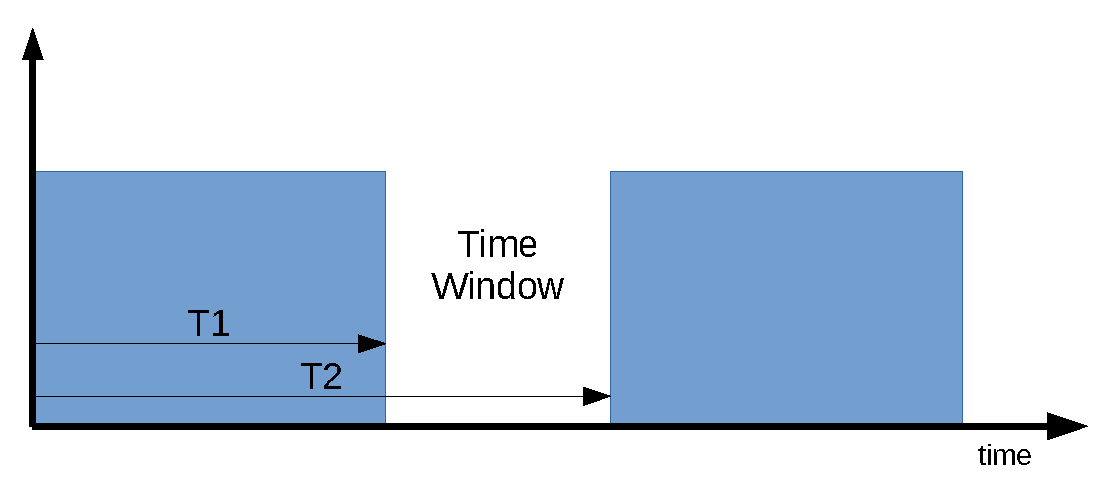
\includegraphics[scale=0.6]{windowed-watchdog-timer.pdf}
\caption{Schematic design of a windowed watchdog timer \cite{elattar2007}.}
\label{fig:windowed-watchdog-timer}
\end{figure}

\item [Sequenced Watchdog Timer.] 
This design is a further improvement of the \emph{Windowed Watchdog Timer} and bases on the same principle. In contrast, to the other designs, the signal sent from the mirrored service carries a sequenced parameter. Only if the signal arrives in time and within the specified time window, this parameter is evaluated and compared to a parameter inside the WDT. If those match the sequence variable in the WDT, the variable gets incremented and the timer reseted, starting the cycle all over again \cite{elattar2007}.
The whole process is illustrated in figure \ref{fig:sequenced-watchdog-timer}.

The disadvantage of this design is the clearly higher complexity, for the \emph{Sequenced Watchdog Timer} must be capable of holding and modifying state information as well as comparing it to received information.

\begin{figure}[!htbp]
\centering
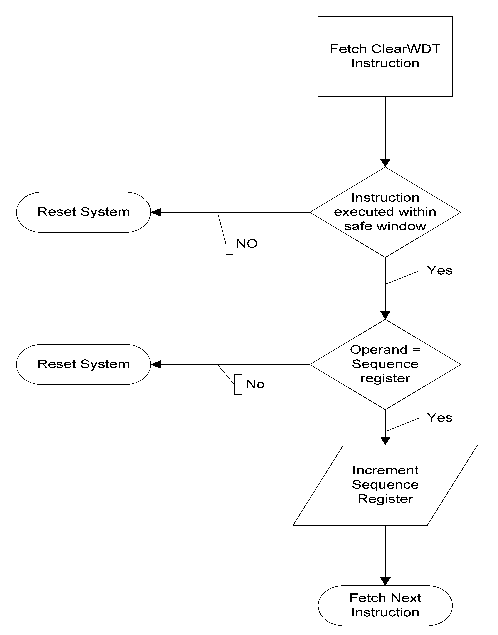
\includegraphics[scale=1.2]{sequenced-watchdog-timer.pdf}
\caption{Schematic illustration of the operational principle of a \emph{Sequenced Watchdog Timer} \cite{elattar2007}.}
\label{fig:sequenced-watchdog-timer}
\end{figure}

\end{description}






\subsection{Error Detection/Masking Service}
\label{sec:error-detection-service}

Most of the errors, especially those which do not alter the timing, remain unnoticed by the WDT. There are several approaches in the design of an error detection service, but the most simple and approved one, is based on triple modular redundancy (TMR). With this approach an error detection service mirrors three individual and independent services, which provide the same functionality (e.g. acceleration measurement). A comparing logic inside the error detection service compares the information received from these services and can identify an error in one of the services by means of a simple voting mechanism \cite{wiki_tmr}. In event of an error, another service can be triggered for restarting the erroneous service or performing other countermeasures.

The very same implementation is also capable of performing \emph{error masking}, because due to the redundancy and the voting system the service could also hide an error in one of the mirrored elements, without the service consumer noticing.


\subsection{Memory Protection}
Memory protection is related to safety as well as security. It is a method for preventing processes or users from accessing memory that is not allocated to them.

Former embedded systems, or such that are small in size, do not necessarily require memory protection mechanisms, because all related programs have a very specific purpose and an unintended behaviour is rather unlikely. In such cases, the overhead in runtime, when using memory protection just does no pay off \cite{yamada2008}. 

Modern, large scale system, on the other hand, dispose of numerous third-party components for the interaction with the user and the environment. At the same time, the overhead in computing is no longer crucial, due to the fast increase in computing power  \cite{yamada2008}. Especially, if the system is connected to a public network like the Internet, memory protection becomes also a big issue for the prevention of malicious attacks.

There are, several other aspects stressing the need for memory protection in ES:

\begin{itemize}
\item It can serve as fault- and error detection and containment mechanism, preventing a failure of one service to propagate and infect the whole system \cite{yamada2008}.
\item It protects the system from unintended behaviour of the particular services \cite{yamada2014}.
\item It is an important aid for the development process and helps at debugging by identifying ``illegal'' behaviour of erroneous services, resulting in a reduced development time \cite{yamada2008} \cite{yamada2014}.
\end{itemize}

As a service, it could be implemented like the \emph{Information Assurance} core service from the Arrowhead framework (cf. section \ref{ch:system_layers}), with dedicated services for authentication, granting privileges and managing authorization information.


\subsection{Requirements Validation Service}

This service should be responsible for checking the compliance of safety margins, when services are composed. For example, if a service is required to be in compliance with ASIL D, it cannot be based on another service, which can only provide ASIL B. According to its specification the requirements validation service could either prevent this orchestration, or even look for possible solutions, e.g. looking for a service with the same functionality and ASIL D, or combining two of the ASIL B services.

A service like this is surprisingly nowhere mentioned throughout literature, but according to various findings this is a crucial mechanism, in order to do not violate functional safety requirements, when composing services.








\section{Service development process}
\label{sec:service-development-process}
In order to be in compliance with given design rules and standards, the development of services has to follow strict protocols.

The development stages considered in this section are an adoption of the development stages, provided by Erl et al. in \cite[p.116]{erl2011}. In detail, the first four stages are the object of investigation. The stages are renamed to fit for the development of a single service instead of an overall SoA and are denominated:
\begin{itemize}
\item \emph{Service investigation/planning},
\item \emph{Service inventory analysis},
\item \emph{Service oriented analysis} and
\item \emph{Service oriented design} \cite[p.116]{erl2011}.
\end{itemize}


\subsection{Service Investigation/Planning}
This phase is concerned with the initial layout of the service. It is the phase where necessary requirements are listed and explored. There are several questions which need to be answered during this stage:
\begin{itemize}
\item What is the scope of the service?
\item What are required capabilities?
\item Which capabilities are not required?
\item What are the safety requirements concerning this service?
\item Should this functionality be implemented as service at all?
\end{itemize}



\subsection{Service Inventory Analysis}

During the service inventory analysis the service inventory (cf. section \ref{sec:structure_of_soa}) is searched for services which are required in order to build up the desired service. This simplifies the development, because much of the required functionality is already provided by other services and at the same time this step is responsible for preventing redundancies.

The outcome of the service inventory analysis phase is a so called \emph{service candidate}. This denotes a conceptual service model before it is implemented by means of a specific language. According to \cite[p.42]{erl2011}, the concept of a language independent service candidate is applied, because the service undergoes a lot of changes in these early stages of development. Nevertheless, this may not be practicable in reality and it is not unlikely that the templates for the service contract are used and extended from the very beginning of the development process.

\subsection{service oriented analysis}

During the service oriented analysis phase the service candidate is reviewed and checked in terms of \emph{naming} and \emph{normalisation}.

\begin{description}
	\item [Service naming.]
	The naming of the service candidate must be in accordance with other, existing, services \cite[p.206]{erl2011}.

	In terms of automotive, the naming is governed by certain standards, like \mbox{AUTOSAR}, which proposes naming conventions in their \textbf{SW-C and System Modelling Guide} \cite{autosar_system_modelling}.

	A unified naming convention is quite helpful, when dealing with standardised interfaces and provides a possibility to include relevant meta data, like the related system or intended functionality, into the name \cite{rehner2013}.

	\item [Service normalisation.]
	Services within the same service inventory shall not have overlapping boundaries. In other words, redundant logic should generally be avoided, for it would violate the concept of a SoA. Accordingly, the services are forced to use existing services if those offer the required functionality \cite[p.207]{erl2011}.

	\item [Service Candidate Review.]
	The final phase of this stage is a review by the related developers. A possible outcome of this review is the approval of changes or extensions to the service candidate \cite[p.210]{erl2011}.

	In order to ensure an unbiased outcome, this review could be conducted by ``external'' people, which have not been included into the development process up to this step, but still have a thorough knowledge of the SoA principles. Those people might think of a quite different approach for the very same problem and could raise new questions concerning the proposed design and composition.

	A review can also take place if an existing and already implemented service is extended by one or more new capabilities \cite[p.210]{erl2011}.
\end{description}




\subsection{service oriented design}

Erl et al. \cite[p.86]{erl2011} describe this phase as:
\begin{quote}
``Service-Oriented Design subjects this service candidate to additional considerations that shape it into a technical service contract in alignment with other service contracts being produced for the same service inventory.''
\end{quote}


The aim of the service oriented design phase is to physically establish the service contract by filling out the corresponding templates. It is initiated when sufficient analysis has been conducted and ends with a finished service contract as output.








\section{Use Case Scenario}

As final part of this investigation, a short use case scenario was conducted. In detail, the development process of an \emph{error detection service} was investigated by means of the development phases featured in section \ref{sec:service-development-process}. Due to the scarce reference material related to this topic, the use case scenario is rather short and quite theoretical. However, it provides a good example on what the development process of a service may look like.

\subsection{Service Investigation/Planning}


\begin{description}
\item [Scope of the service.]
The service should be capable of detecting an error within a given ECR and act accordingly. Therefore it needs the signal of all the sensors it should mirror, as well as clock signal for creating sampling times.
\item [Required capabilities.]
	\begin{itemize}
	\item Detection an error in one of the sensors.
	\item Restart of an erroneous sensor.
	\item Purging the service from the service repository if more than two sensors fail and errors can no longer be detected.
	\end{itemize}
\item [Non-required capabilities.]
	\begin{itemize}
	\item Detection of a fault.
	\item Detection of a failure.
	\end{itemize}
\end{description}



\subsection{Service Inventory Analysis}


The error detection service will require:
\begin{itemize}
\item A \emph{clock service} for creating sampling times,
\item A \emph{fault detection service} for detecting a fault in one of the mirrored services,
\item A \emph{management service for the service repository} to update the repository in case of an erroneous service, and additionally perhaps
\item A \emph{service for restarting another service}, which is erroneous.
\end{itemize}

During operation, it will also need the redundant service inside the ECR, whose functionality shall be checked for errors. Of course they should feature different implementations on independent hardware components, so that an error could not emerge in multiple services at the same time.


\subsection{Service Oriented Analysis}


Concerning the naming, the example service should be in accordance with the \mbox{AUTOSAR} naming conventions \cite{autosar_system_modelling}. Hence, a suitable candidate would be \textbf{error\_detection}.

The \emph{service normalisation} and \emph{service candidate review} are not really doable just theoretically. Therefore, it shall be assumed that the example service has no overlapping functionality and has passed the review.





\subsection{Service Oriented Design}

Unfortunately, the service contract templates, which are designed by Arrowhead, were not yet available at the time this thesis was written. Accordingly, there could be no example contract be established.


\subsection{Possible Implementation}

At the end of the first four phases, which are concerned with the conceptual development, the service contract is issued. Subsequently follows the actual implementation of the service by a developer, who was (most likely) not included in the preceding design phases. Therefore, the contract must provide all the necessary information for the implementation process, leaving no ambiguities or open questions.

It is then up to the developer to decide how the service will be implemented, e.g. which programming language or approach to use. The outcome is a certain architecture, which can be based on any arbitrary technology. 

A possible architecture resulting from the service of this use case is a triple modular redundancy approach (cf. section \ref{sec:error-detection-service}), as depicted in figure \ref{fig:example-service-architecture}. 


\begin{figure}[ht]
\centering
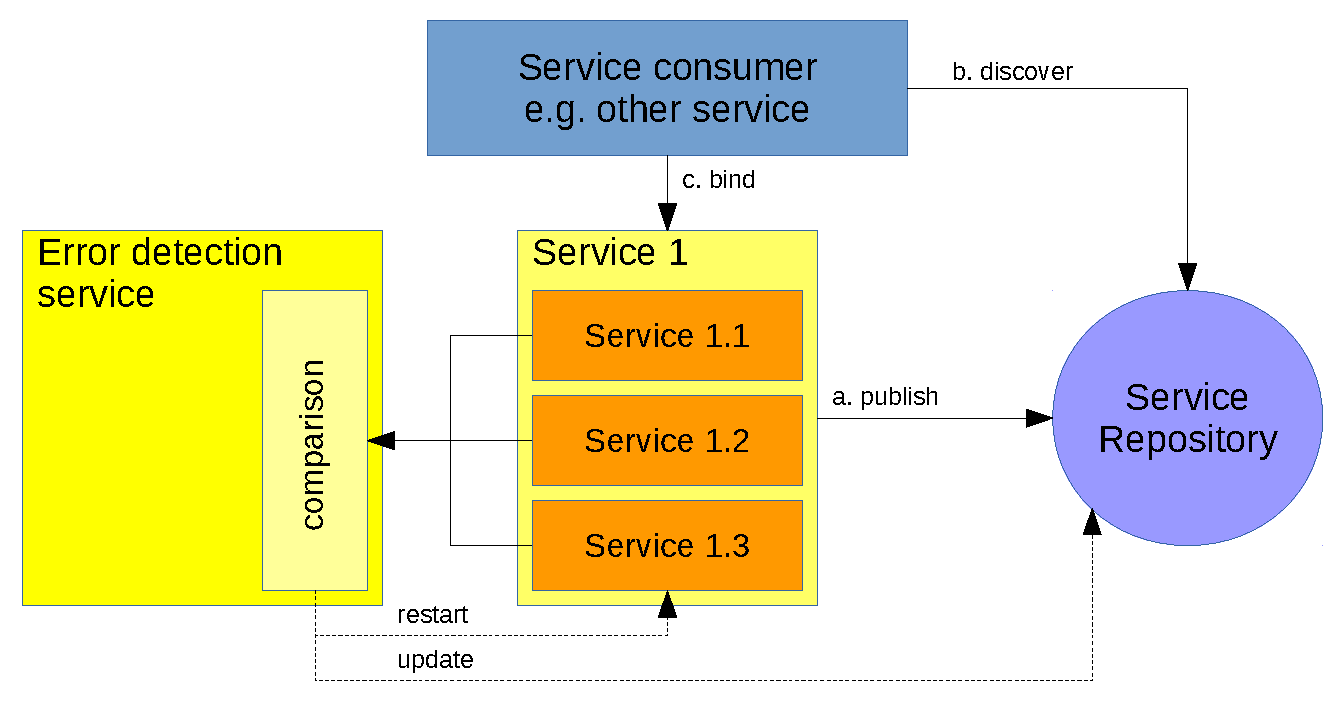
\includegraphics[width=\textwidth]{error-detection-service.pdf}
\caption{Possible architectural implementation of the example service.}
\label{fig:example-service-architecture}
\end{figure}
